\chapter{Diseño e implementación del sistema}
\label{cap:diseno}

Este capítulo describe el sistema tal como quedó construido: los datos que usa,
la cadena de procesamiento que va desde el registro sísmico continuo hasta la
clase de cada evento, y la forma en que se evalúa cada etapa. Los resultados
medidos se presentan en el Capítulo~\ref{cap:resultados}.

\section{Datos}
\label{sec:datos}

Un sismómetro registra el movimiento del suelo de forma continua. Cada
estación tiene tres componentes: una vertical (Z) y dos horizontales, norte--sur
(N) y este--oeste (E). La señal se guarda como una secuencia de valores tomados
100 veces por segundo (100\,Hz). En este trabajo se usa una sola estación del
Complejo Volcánico Nevados de Chillán, llamada FRE, con sus tres componentes.

\subsection{Traza continua de evaluación}
\label{subsec:traza}

La traza continua es un registro de 10,18 horas publicado junto con el
conjunto de datos de \textcite{espinosacurilem2025dataset}. Une tres tramos
de fechas distintas: 6 horas del 9 de febrero de 2018, 3 horas del 14 de enero
de 2020 y 1,18 horas del 10 de enero de 2017. Trae un catálogo de 205 eventos,
cada uno con su inicio, su fin y su clase. Las clases son cinco. Tres son
volcánicas: los volcano-tectónicos (VT), que son fracturas de roca bajo el
volcán; los de largo período (LP), asociados al movimiento de fluidos; y el
tremor (TR), una vibración sostenida que puede durar minutos. Dos no son
volcánicas: las avalanchas (AV) y los ice-quakes (IC), que son fracturas del
hielo del glaciar. Las métricas principales de este trabajo usan solo VT, LP y
TR; AV e IC se agrupan en una clase llamada \emph{rechazo}.

La traza publicada contiene solo la componente vertical de varias estaciones.
Para tener Z, N y E reales de FRE se usaron los registros originales de la
estación (``crudos''), que se alinearon con la traza publicada comparando la
componente vertical de ambos (correlación cruzada) en cada tramo. Los crudos
tienen huecos; quedan 9,74 horas válidas con las tres componentes. Diecisiete
avalanchas del primer tramo no tienen señal en el crudo y no se usan. Los
eventos volcánicos que se evalúan son 125: 36 VT, 52 LP y 37 TR.

La traza continua se usa solo para evaluar el sistema completo. Ningún dato de
ella se usa para entrenar ni para ajustar parámetros.

\subsection{Ventanas etiquetadas para entrenar y probar el clasificador}
\label{subsec:ventanas}

El clasificador se entrena con ventanas de 300\,s del registro continuo de FRE,
cada una centrada en un evento catalogado. Los eventos provienen del conjunto
publicado por \textcite{espinosacurilem2025dataset} y de su catálogo de
Nevados de Chillán. Cada ventana trae ``cajas'': el inicio, el fin y la clase
de cada evento del catálogo que cae dentro de ella. La caja del evento que
centra la ventana se llama \emph{principal}; las de los demás eventos que
aparecen en la misma ventana se llaman \emph{extra}. El conjunto de ventanas
excluye los eventos de más de 300\,s, los de clase ambigua y las ventanas que
se cruzan en el tiempo con la traza continua.

Las ventanas vienen separadas en dos grupos: \emph{desarrollo}, para entrenar
y validar, dividido a su vez en cinco partes (\emph{folds}), y \emph{test},
que se reserva para la evaluación final. Separar por ventana, y no por evento
recortado, evita que recortes de una misma ventana queden a la vez en
entrenamiento y en evaluación.

Para cada ventana se extrajeron Z, N y E de FRE desde la base de datos del
registro continuo. Se usan solo las ventanas con las tres componentes
completas: 5.669 (4.508 de desarrollo y 1.161 de test). Como comprobación, se
verificó que ninguna de estas ventanas comparte tiempo con la traza continua.

\section{Arquitectura de la cadena}
\label{sec:arquitectura-cadena}

El sistema se organiza como una cadena de cinco etapas, que muestra la
Figura~\ref{fig:arquitectura}. La misma cadena se aplica a las ventanas
etiquetadas, para entrenar y probar el clasificador, y a la traza continua,
para evaluar el sistema completo.

\begin{figure}[!ht]
\centering
\begin{tikzpicture}[
  font=\footnotesize,
  etapa/.style={draw, rectangle, rounded corners=2pt, align=center,
    minimum height=1.0cm, minimum width=7.2cm, inner sep=4pt},
  flujo/.style={-{Stealth[length=2.5mm]}, thick},
  etiq/.style={font=\scriptsize, align=left}]
\node[etapa] (a) {\textbf{1. Detección}\\PhaseNet sobre Z, N y E filtradas en 1--15\,Hz};
\node[etapa, below=0.85cm of a] (b) {\textbf{2. Recorte}\\inicio y fin de cada evento por la energía de la señal};
\node[etapa, below=0.85cm of b] (c) {\textbf{3. Espectrograma}\\imagen tiempo--frecuencia de Z, N y E};
\node[etapa, below=0.85cm of c] (d) {\textbf{4. Clasificación}\\red convolucional: VT, LP, TR o rechazo};
\node[etapa, below=0.85cm of d] (e) {\textbf{5. Evaluación}\\comparación con el catálogo};
\node[above=0.6cm of a, etiq, align=center] (in) {registro continuo de FRE};
\draw[flujo] (in) -- (a);
\draw[flujo] (a) -- node[etiq, right=3pt] {avisos de llegada de ondas} (b);
\draw[flujo] (b) -- node[etiq, right=3pt] {intervalos recortados} (c);
\draw[flujo] (c) -- node[etiq, right=3pt] {imagen de 224\,$\times$\,224} (d);
\draw[flujo] (d) -- node[etiq, right=3pt] {clase y probabilidades} (e);
\end{tikzpicture}
\caption{Etapas de la cadena de procesamiento.}
\label{fig:arquitectura}
\end{figure}

\subsection{Datos que pasan de una etapa a otra}
\label{sec:contrato-datos}

Cada etapa deja un archivo que la siguiente lee, de modo que cualquier cifra
del informe se puede regenerar desde esos archivos. La detección deja los
avisos, con la fase (P o S), el instante y la probabilidad. El recorte deja
cada intervalo con su inicio y su fin en muestras de la señal. El etiquetado
deja, por recorte, la caja del catálogo que le corresponde, su IoU y su
etiqueta. El espectrograma deja los valores en decibelios de cada ventana. La
clasificación deja, por recorte, la clase elegida y la probabilidad de cada
clase, junto con un registro de la configuración usada, las versiones de las
librerías y las métricas de cada época de entrenamiento.

\section{Detección}
\label{sec:deteccion}

Un detector recorre la señal continua y avisa dónde parece haber un evento.
Se compararon tres (objetivo específico OE1, evaluar detectores): STA/LTA, un
método clásico que compara la energía reciente de la señal con la de un
periodo más largo \parencite{allen1978stalta}, y dos redes neuronales ya
entrenadas, PhaseNet \parencite{zhu2019phasenet} y EQTransformer
\parencite{mousavi2020eqtransformer}, usadas a través de la librería SeisBench
\parencite{woollam2022seisbench} con sus pesos ``original''. Ninguna de las
dos redes se reentrenó. La comparación y la elección se presentan en el
Capítulo~\ref{cap:resultados}; el sistema usa PhaseNet.

PhaseNet recibe Z, N y E y entrega, para cada instante, la probabilidad de que
en ese momento llegue una onda P (la primera onda de un sismo) y la de que
llegue una onda S (la segunda, más lenta). No entrega el fin del evento. Solo
se ajustan los parámetros que expone la propia librería: P\_threshold y
S\_threshold, la probabilidad mínima para considerar que llegó una onda P o S;
overlap, cuántas muestras se traslapan los tramos que la red analiza por
separado (1.500); blinding, cuántas muestras de cada borde de esos tramos se
descartan (250 por lado); y stacking, cómo se combinan los tramos traslapados
(promedio). La señal se filtra antes en 1--15\,Hz, porque PhaseNet no filtra
por su cuenta. La configuración usada es P\_threshold 0,40 y S\_threshold
0,05.

Cada vez que la probabilidad de P o de S supera su umbral se registra un
\emph{aviso} en el punto más alto de esa subida. Los avisos a 5\,s o menos
uno de otro se juntan en uno, porque suelen ser las ondas P y S de un mismo
evento.

La traza continua se entrega a PhaseNet en ventanas de 300\,s que avanzan de a
55\,s. Como el evento más largo del catálogo dura 240,8\,s, todo evento
queda completo dentro de al menos una ventana.

\section{Recorte por energía}
\label{sec:recorte}

PhaseNet dice dónde empieza un evento, pero no dónde termina. Para delimitarlo
se usa un recorte por energía, un método propio pedido por el profesor guía,
que sigue estos pasos:

\begin{enumerate}
\item Se calcula la \emph{envolvente} de la señal: en cada instante, la raíz
  de la energía promedio de Z, N y E durante el segundo que lo rodea.
\item Se mide el nivel del ruido antes del evento: el percentil 20 de la
  envolvente entre 120\,s y 5\,s antes del aviso. El percentil 20 se elige
  porque no lo altera la cola de un evento anterior. En las ventanas
  etiquetadas, ese periodo se toma solo dentro de la ventana.
\item El recorte empieza 2,5\,s antes del aviso, margen que cubre el error de
  inicio medido en la detección (entre 1,7 y 2,4\,s).
\item El recorte termina donde empieza el primer tramo de 5\,s en que la
  envolvente se mantiene bajo el doble del nivel del ruido, buscando entre 2 y
  300\,s después del aviso.
\item Si antes de ese fin llega otro aviso, el recorte se corta 2,5\,s antes
  de ese aviso, para no mezclar dos eventos.
\end{enumerate}

El recorte no usa ninguna información del catálogo: solo la señal y los
avisos de PhaseNet.

\section{Etiquetado de los recortes}
\label{sec:etiquetado}

Para entrenar y evaluar, cada recorte recibe una etiqueta según cuánto se
parece a una caja del catálogo. La medida es el IoU (\emph{intersection over
union}): el tiempo que el recorte y la caja tienen en común, dividido por el
tiempo total que cubren entre los dos. Vale 1 si coinciden exactamente y 0 si
no se tocan. Recortes y cajas se emparejan de a uno, empezando por los pares
de mayor IoU. Con ese emparejamiento:

\begin{itemize}
\item si el IoU es 0,3 o más, el recorte toma la clase de la caja; AV e IC
  pasan a la clase de rechazo;
\item si el recorte toca alguna caja pero con IoU menor, se marca ``fuera'' y
  no se usa, porque su delimitación es demasiado mala para asignarle una
  clase;
\item si no toca ninguna caja, se marca ``sin caja''. Puede ser una falsa
  alarma del detector o un evento que el catálogo no registra. No se usa para
  entrenar ni en las métricas del clasificador; solo se cuenta cuántos de ellos
  el clasificador llama volcánicos.
\end{itemize}

Sobre las 5.651 ventanas etiquetadas que tienen al menos un recorte, el
detector y el recorte producen 37.228 recortes, que se reparten como muestra
el Cuadro~\ref{tab:recortes-folds}.

{\small
\begin{longtable}{lrrrrrrrr}
\caption{Recortes de las ventanas etiquetadas por etiqueta y por parte del
conjunto.}\label{tab:recortes-folds}\\
\toprule
\textbf{Etiqueta} & \textbf{Fold 1} & \textbf{Fold 2} & \textbf{Fold 3} &
\textbf{Fold 4} & \textbf{Fold 5} & \textbf{Test} & \textbf{Total} \\
\midrule
\endfirsthead
\toprule
\textbf{Etiqueta} & \textbf{Fold 1} & \textbf{Fold 2} & \textbf{Fold 3} &
\textbf{Fold 4} & \textbf{Fold 5} & \textbf{Test} & \textbf{Total} \\
\midrule
\endhead
\bottomrule
\endlastfoot
VT & 245 & 235 & 240 & 262 & 256 & 336 & 1.574 \\
LP & 563 & 541 & 512 & 514 & 520 & 676 & 3.326 \\
TR & 210 & 203 & 221 & 200 & 188 & 244 & 1.266 \\
AV & 94 & 103 & 104 & 95 & 102 & 133 & 631 \\
IC & 123 & 151 & 142 & 127 & 145 & 191 & 879 \\
Fuera & 1.063 & 1.141 & 1.116 & 1.033 & 1.042 & 1.355 & 6.750 \\
Sin caja & 3.629 & 3.519 & 3.551 & 3.650 & 3.767 & 4.686 & 22.802 \\
\midrule
Total & 5.927 & 5.893 & 5.886 & 5.881 & 6.020 & 7.621 & 37.228 \\
\end{longtable}
}

\section{Espectrogramas}
\label{sec:recorte-espectrogramas}

El clasificador no recibe la señal, sino una imagen de ella: el
\emph{espectrograma}, que muestra cómo se reparte la energía de la señal entre
las frecuencias a lo largo del tiempo. El eje horizontal es el tiempo, el
vertical la frecuencia y el color la energía, en decibelios (dB), una escala
logarítmica.

Los espectrogramas se calculan sobre la ventana de 300\,s completa, con los
mismos parámetros con que se prepararon las ventanas etiquetadas: la señal se
filtra entre 1 y 15\,Hz con un filtro Butterworth de orden 15 aplicado hacia
adelante y hacia atrás, para no desplazarla en el tiempo; el espectrograma se
calcula en tramos de 256 muestras (2,56\,s) que avanzan de a 64, con ventana
de Hann y 512 puntos de frecuencia, y se conservan las frecuencias de 0 a
15\,Hz. Resultan 77 filas de frecuencia y 465 columnas de tiempo por ventana,
una columna cada 0,64\,s.

Los colores siguen la escala \emph{jet}, que va del azul oscuro al rojo. El
rojo corresponde a la energía máxima de cada componente en la ventana y el
azul más oscuro a 60\,dB bajo ese máximo; lo que queda más abajo se ve del
mismo azul. Z, N y E se apilan una sobre otra, de modo que cada imagen tiene
231 filas.

La imagen de un recorte son las columnas de la ventana que caen dentro de él.
Como los eventos duran distinto, las imágenes tienen anchos distintos, y las
redes necesitan una entrada de 224\,$\times$\,224 píxeles, el tamaño con que
fueron preentrenadas. Cada imagen se redimensiona a ese tamaño con
interpolación bilineal: se estira si tiene menos de 224 columnas y se comprime
si tiene más, sin cortar nada. No se usa el recorte central que traen las
redes por defecto, porque cortaría el inicio y el fin del evento. La
Figura~\ref{fig:estiramiento} muestra el proceso con un recorte corto y uno
largo.

\begin{figure}[!ht]
\centering
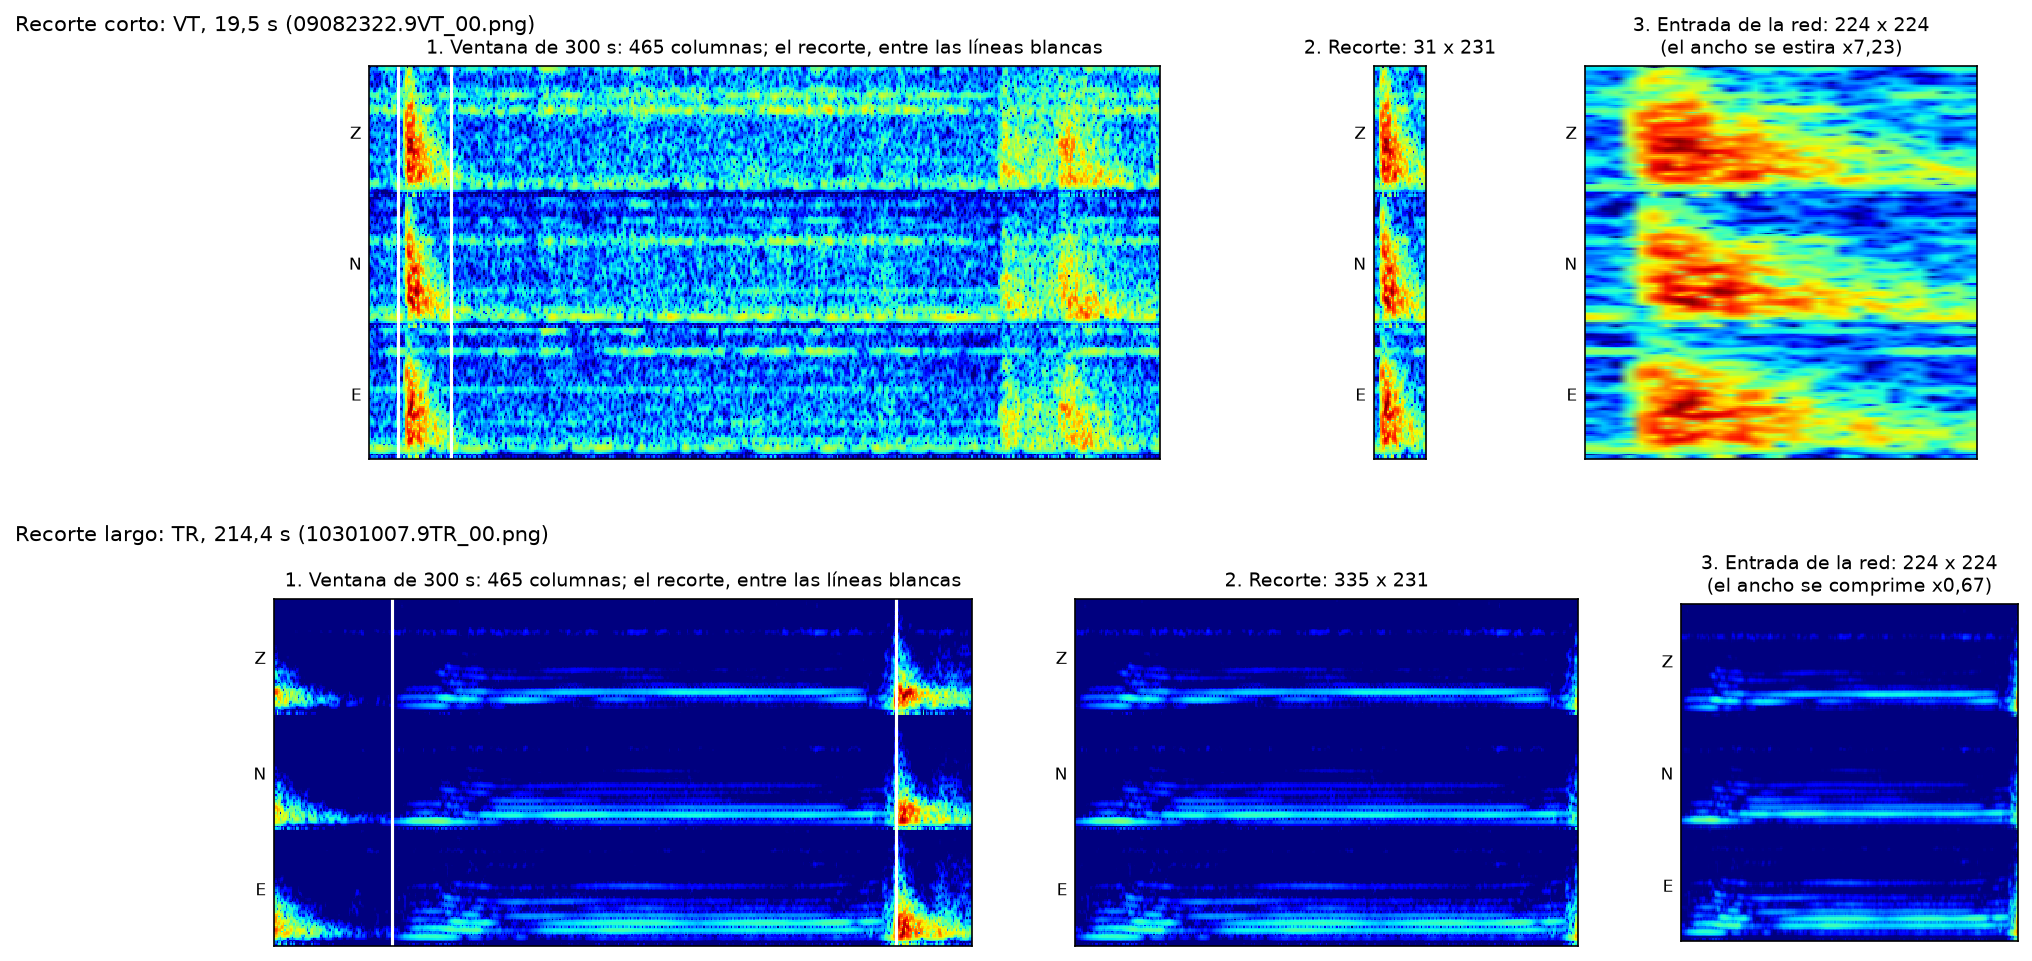
\includegraphics[width=\textwidth]{images/figura_estiramiento.png}
\caption{Del recorte a la entrada de la red. Arriba, un VT de 19,5\,s
(31 columnas), que se estira 7,23 veces; abajo, un TR de 214,4\,s
(335 columnas), que se comprime a 0,67. En cada fila: la ventana de 300\,s con
el recorte entre las líneas blancas, el recorte a su tamaño y la imagen de
224\,$\times$\,224 que recibe la red.}
\label{fig:estiramiento}
\end{figure}

Los recortes de menos de 5\,s se dejan fuera: al estirarlos, unas pocas
columnas se repiten decenas de veces y la imagen queda reducida a franjas
horizontales.

Como alternativa, el profesor guía pidió probar una duración fija: desde el
inicio de cada recorte se toman 60\,s de la ventana, sin importar cuánto dure
el evento. Si no alcanzan dentro de la ventana, se toman sus últimos 60\,s.
Estos resultados se muestran aparte, sin compararlos directamente con los del
recorte.

\section{Clasificador por transferencia de aprendizaje}
\label{sec:clasificador-transferencia}

\subsection{Redes}

Una red neuronal convolucional aprende a reconocer patrones en imágenes. En
vez de entrenarla desde cero, lo que requeriría muchas más imágenes, se parte
de una red ya entrenada con ImageNet, una colección de más de un millón de
fotografías de objetos comunes, y se ajusta a este problema \parencite{deng2009imagenet}. Esto se llama
\emph{transferencia de aprendizaje}: lo que la red aprendió a reconocer en
fotografías, como bordes, texturas y formas, sirve de punto de partida para
los espectrogramas.

Se comparan tres redes, todas de la librería torchvision con sus pesos
preentrenados por defecto: VGG16 \parencite{simonyan2015vgg}, que es la usada
por \textcite{espinosacurilem2025ood} en este mismo volcán; ResNet50
\parencite{he2016resnet}; y EfficientNet-B0 \parencite{tan2019efficientnet},
una red liviana. En las tres se reemplaza la última capa por una nueva con
cuatro salidas, una por clase: VT, LP, TR y rechazo. Se ajusta la red completa,
no solo la capa nueva. Las imágenes se normalizan con la media y la desviación
de ImageNet, igual que al preentrenar.

\subsection{Entrenamiento}

El entrenamiento muestra a la red las imágenes de cuatro folds y ajusta sus
pesos para que acierte la clase; el quinto fold se usa para validar, es decir,
para medir cómo le va con imágenes que no vio. Una pasada completa por las
imágenes de entrenamiento se llama \emph{época}. Los elementos que se ajustan
son los siguientes; todos son parámetros de PyTorch o torchvision
\parencite{paszke2019pytorch} y parten de su valor por defecto:

\begin{itemize}
\item Optimizador, el método que actualiza los pesos: AdamW
  \parencite{loshchilov2019adamw} o descenso de gradiente estocástico (SGD)
  con momentum 0,9.
\item Tasa de aprendizaje, el tamaño de cada ajuste de los pesos.
\item Weight decay, una penalización que evita pesos demasiado
  grandes.
\item Dropout, que durante el entrenamiento apaga al azar una
  fracción de las neuronas de las últimas capas para que la red no dependa de
  unas pocas \parencite{srivastava2014dropout}. VGG16 y EfficientNet-B0 lo
  traen como parámetro; a ResNet50, que no lo tiene, se le agrega una capa de
  dropout antes de la capa nueva.
\item Tamaño de lote, cuántas imágenes se usan en cada ajuste.
\item Función de pérdida, la medida del error que se minimiza. Se
  prueban dos: la entropía cruzada, con cada clase pesada por el inverso de su
  frecuencia para que las clases con menos ejemplos cuenten lo mismo, y la
  pérdida focal \parencite{lin2017focal}, que da más peso a los ejemplos
  difíciles, con sus valores por defecto en torchvision.
\end{itemize}

Las imágenes ``sin caja'' no se usan en el entrenamiento: la clase de rechazo
se forma solo con AV e IC.

Para decidir cuándo parar, después de cada época se mide en el fold de
validación el F1 macro de VT, LP y TR (definido en la
Sección~\ref{sec:protocolo}). Si no mejora durante 5 épocas seguidas, el
entrenamiento se detiene, con un máximo de 50 épocas. Se conservan los pesos de
la mejor época.

\subsection{Aumento de datos}
\label{subsec:aumento}

El aumento de datos modifica al azar las imágenes de entrenamiento en cada
época, para que la red vea variaciones de un mismo evento y no memorice las
imágenes exactas. Se aplica solo en el entrenamiento; la validación y el test
usan siempre las imágenes sin modificar. Se usan dos variaciones:

\begin{itemize}
\item Rango de colores. En vez de cambiar los colores de la imagen
  ya hecha, se cambia el rango en dB con que se colorea el espectrograma: el
  máximo se corre al azar entre $-5$ y $+5$\,dB y el ancho del rango se elige
  al azar entre 50 y 70\,dB, igual para las tres componentes. Así el mismo
  evento aparece con sus componentes más o menos marcadas, como un evento con
  más o menos ruido. La Figura~\ref{fig:rangos} muestra el efecto con límites
  más amplios que los usados.
\item Deformación elástica, que desplaza suavemente los píxeles de
  la imagen \parencite{simard2003elastic}, con la función ElasticTransform de
  torchvision y sus valores por defecto (alpha 50 y sigma 5). Se aplica solo
  en el eje del tiempo, porque deformar la frecuencia cambiaría justamente lo
  que distingue a un LP de un VT. La Figura~\ref{fig:elastica} compara las dos
  opciones.
\end{itemize}

No se usa el recorte aleatorio de la imagen, porque podría quitar el inicio o
el fin del evento. Los límites del rango de colores y la elección del eje de la
deformación son decisiones propias de este trabajo.

\begin{figure}[!ht]
\centering
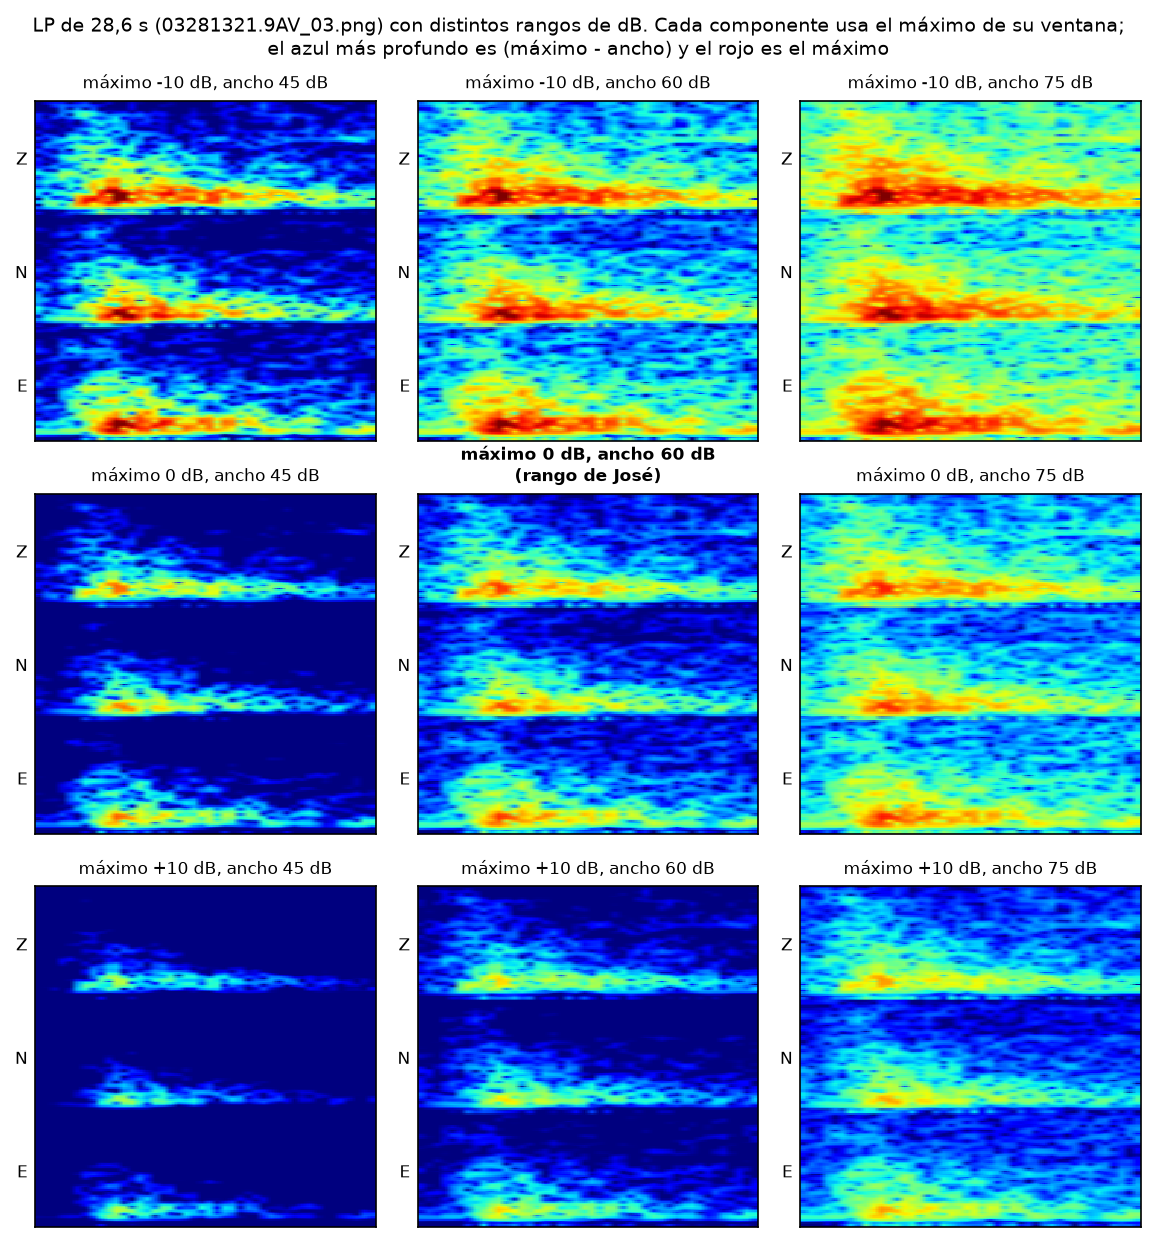
\includegraphics[width=0.85\textwidth]{images/figura_rangos_db.png}
\caption{Un mismo LP coloreado con distintos rangos de dB. Al centro, el rango
de las imágenes sin aumento: el máximo de cada componente y 60\,dB bajo él.
En el entrenamiento se usan corrimientos de hasta 5\,dB y anchos entre 50 y
70\,dB.}
\label{fig:rangos}
\end{figure}

\begin{figure}[!ht]
\centering
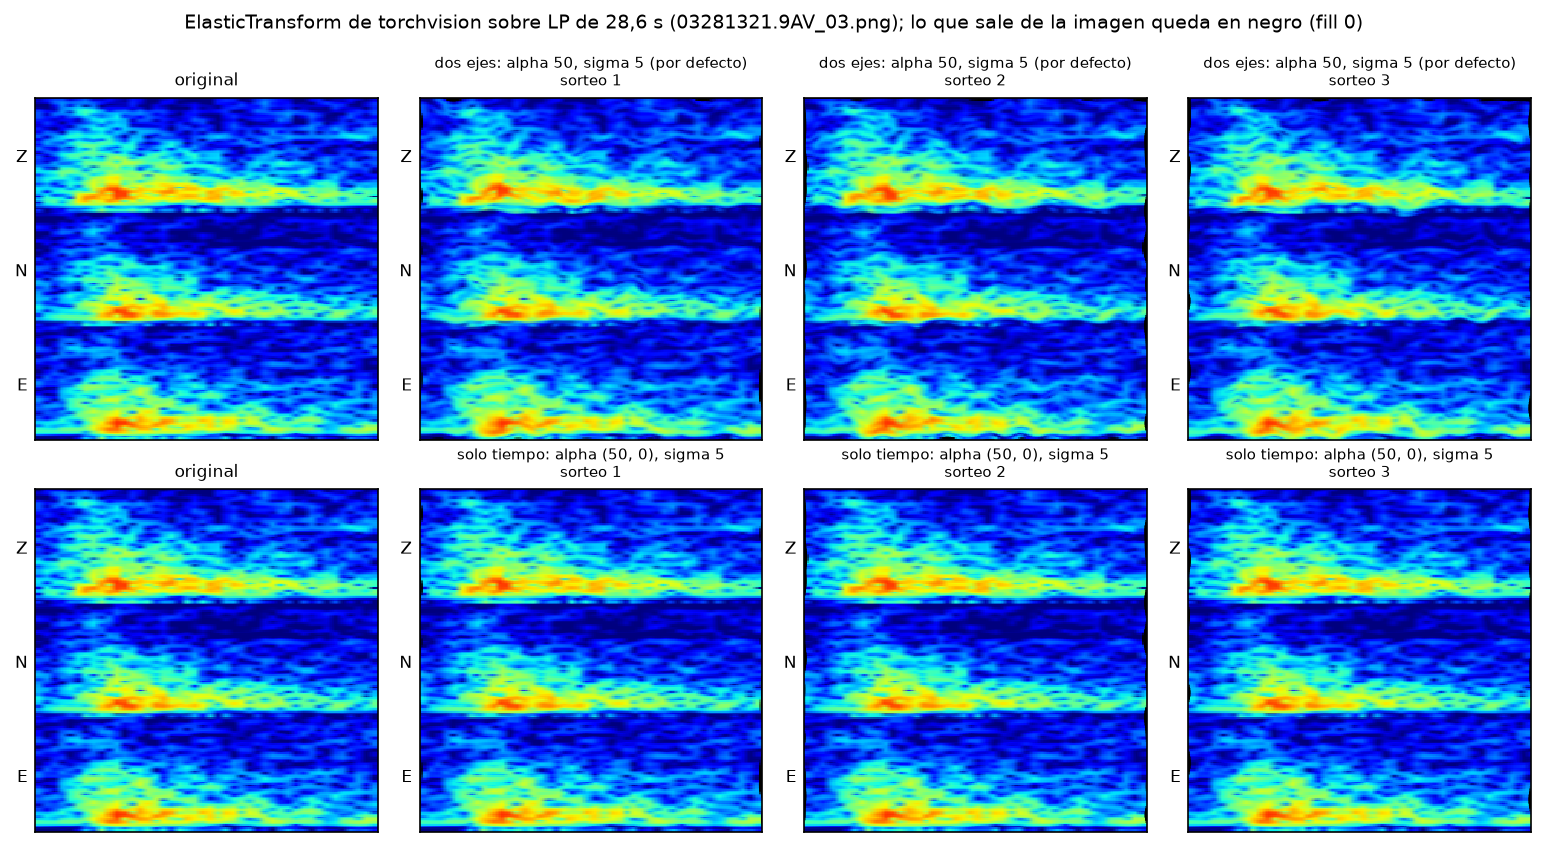
\includegraphics[width=\textwidth]{images/figura_elastica.png}
\caption{Deformación elástica sobre el mismo LP. Arriba, en los dos ejes: las
líneas de frecuencia se ondulan. Abajo, solo en el eje del tiempo, que es la
opción usada: las frecuencias quedan en su lugar.}
\label{fig:elastica}
\end{figure}

\subsection{Búsqueda de la configuración}
\label{subsec:busqueda}

Para elegir la combinación de parámetros de cada red se hace una búsqueda
bayesiana con Optuna \parencite{akiba2019optuna}, con su método por defecto,
TPE \parencite{bergstra2011tpe}. En vez de probar todas las combinaciones, que
serían 128 por red, este método mira cómo resultaron las pruebas anteriores y
propone las siguientes en las zonas que funcionaron mejor. Se hacen 20 pruebas
por red, entrenando con los folds 2 a 5 y validando con el fold 1, y se elige
la combinación con mayor F1 macro de VT, LP y TR en validación. El
Cuadro~\ref{tab:espacio} muestra los valores probados.

{\small
\begin{longtable}{>{\raggedright\arraybackslash}p{4.2cm}>{\raggedright\arraybackslash}p{7.2cm}}
\caption{Valores probados en la búsqueda de la configuración.}\label{tab:espacio}\\
\toprule
\textbf{Parámetro} & \textbf{Valores} \\
\midrule
\endfirsthead
\toprule
\textbf{Parámetro} & \textbf{Valores} \\
\midrule
\endhead
\bottomrule
\endlastfoot
Optimizador & AdamW; SGD con momentum 0,9 \\
Tasa de aprendizaje & 0,01; 0,001; 0,0001; 0,00001 \\
Dropout & 0,2; 0,3 \\
Tamaño de lote & 16; 32 \\
Weight decay & 0; 0,0001 \\
Función de pérdida & entropía cruzada con pesos por clase; pérdida focal \\
\midrule
Fijos & ajuste de la red completa; duración mínima de 5\,s; sin las imágenes
``sin caja''; máximo 50 épocas; parada temprana con paciencia 5; aumento de
datos de la Sección~\ref{subsec:aumento} \\
\end{longtable}
}

\subsection{Validación cruzada y test}

Con la combinación elegida, cada red se entrena cinco veces: en cada una se
valida con un fold distinto y se entrena con los otros cuatro. El mejor modelo
de cada una de esas cinco corridas se evalúa sobre las ventanas de test, que
no participaron en ninguna decisión. Así se obtienen cinco valores de cada
métrica, de los que se informan el promedio, el mínimo, el máximo y la
desviación estándar. Todo se repite con la ventana fija de 60\,s.

El entrenamiento se hizo en un servidor con una GPU NVIDIA RTX 5090 de la
universidad, con PyTorch 2.14 y CUDA 13.0, enviando cada corrida a la cola de
trabajos del servidor (Slurm). La semilla de los generadores de números al azar se fija para que
cada corrida se pueda repetir.

\section{Protocolo de evaluación}
\label{sec:protocolo}

\subsection{Métricas}

Para cada clase se cuentan los aciertos y los errores del sistema contra el
catálogo:

\begin{itemize}
\item Sensibilidad: de los eventos de una clase, la fracción que el
  sistema encuentra o clasifica bien. Es la métrica de la meta del trabajo,
  que es llegar a 0,95.
\item Precisión: de lo que el sistema asigna a una clase, la
  fracción que de verdad es de esa clase.
\item F1: combina las dos anteriores en un solo número (su media
  armónica); es alto solo si ambas lo son.
\item F1 macro de VT, LP y TR: el promedio simple del F1 de las tres
  clases volcánicas, de modo que cada clase pesa lo mismo aunque tenga menos
  ejemplos.
\item Matriz de confusión normalizada por fila: para cada clase real,
  qué fracción de sus eventos se asignó a cada clase. La diagonal es la
  sensibilidad de cada clase y el resto muestra con qué se confunde.
\end{itemize}

No se usa la exactitud global (el porcentaje total de aciertos), porque las
clases tienen tamaños muy distintos: LP reúne cerca de la mitad de los
eventos, y una red podría acertar mucho LP y fallar TR con una exactitud alta.

\subsection{Detección y recorte}

En la comparación de detectores sobre la traza continua, un evento cuenta como
detectado si hay un aviso a 5\,s o menos de su inicio, antes o después, y cada
aviso cuenta para un solo evento; la misma regla se aplica a los tres
detectores. En las ventanas de test, un evento cuenta como detectado si alguno
de los intervalos en que la probabilidad de P o de S de PhaseNet supera su
umbral se cruza con su caja. La calidad del recorte se mide con el IoU contra
la caja, informando qué fracción de los eventos tiene un recorte con IoU de
0,3 o más y de 0,5 o más. Las falsas alarmas se informan como recortes sin
caja por hora de registro, y su proporción entre todos los recortes como FDR
(\emph{false discovery rate}).

\subsection{Sistema completo sobre la traza continua}

El objetivo específico OE4 pide evaluar el sistema integrado sobre registros
continuos. Para eso la cadena completa se aplica a la traza de FRE:

\begin{enumerate}
\item PhaseNet en ventanas de 300\,s que avanzan de a 55\,s, y el recorte por
  energía de la Sección~\ref{sec:recorte}.
\item Para cada recorte, una ventana de 300\,s centrada en él, como las
  ventanas etiquetadas, que tienen su evento principal al centro; sin salir de
  su tramo. Su espectrograma se calcula sobre la señal de FRE sin filtrar,
  para aplicar el mismo filtro y los mismos parámetros que en el entrenamiento,
  y el rango de dB se toma del máximo de esa ventana.
\item Cada recorte se clasifica con los cinco modelos de cada red (uno por
  fold), y se informan el promedio, el mínimo, el máximo y la desviación entre
  los cinco.
\item Los recortes se etiquetan contra el catálogo con la misma regla de la
  Sección~\ref{sec:etiquetado}.
\end{enumerate}

Se informan tres medidas. La primera es la clasificación de los recortes que
calzan con un evento del catálogo (IoU de 0,3 o más). La segunda es la
\emph{sensibilidad completa} de cada clase: la fracción de sus eventos que el
sistema detecta, recorta con IoU de 0,3 o más y clasifica en la clase
correcta, todo a la vez. La tercera son las falsas alarmas por hora que el
clasificador llama volcánicas. Además se mide el tiempo de cada etapa.

Como la traza tiene pocos eventos por clase (entre 24 y 50 recortes que calzan
con un evento), cada sensibilidad se acompaña de su intervalo de confianza de
95\,\% según el método de \textcite{wilson1927}, para distinguir las
diferencias reales de las que se deben al tamaño de la muestra.
